% ==============================================================================
%  Fractal Gravity on Nested S^3 Shells
%  A Minimal-Parameter, Falsifiable Quantum-Gravity Framework
%
%  Final Submission to Physical Review D — 22 June 2025
%  (c) A. Preece & B. Batenin
% ==============================================================================

\documentclass[
  10pt,prd,aps,twocolumn,superscriptaddress,
  nofootinbib,floatfix,tightenlines
]{revtex4-2}

% ---------------------------- Packages --------------------------------
\usepackage[T1]{fontenc}
\usepackage{amsmath,amssymb,mathtools,bm}
\usepackage{graphicx}
\usepackage{mathrsfs}
\usepackage{booktabs}
\usepackage{siunitx}
  \sisetup{
    range-phrase         = --,
    range-units          = single,
    separate-uncertainty = true,
    per-mode             = symbol
  }
\usepackage{pgfplots}
  \pgfplotsset{compat=1.18}
\usepackage{enumitem}
\usepackage{filecontents}
\usepackage{hyperref}
  \hypersetup{
    colorlinks,
    allcolors=blue,
    pdftitle={Fractal Gravity on Nested S^3 Shells},
    pdfauthor={A. Preece and B. Batenin},
    pdfsubject={Theoretical Physics}
  }
\usepackage{cleveref} % Must be loaded after hyperref

% ---------------------------- Macros -----------------------------------
% Physical Constants & Parameters
\newcommand{\GN}{G_{\mathrm{N}}}
\newcommand{\ellP}{\ell_{\mathrm{P}}}
\newcommand{\phig}{\varphi_{\mathrm{g}}} % Golden Ratio

% Operators & Math
\newcommand{\Fop}{\mathscr{F}}
\newcommand{\BOX}{\Box}
\newcommand{\dd}{\mathrm{d}} % Upright d for differentials

% PPN Parameters
\newcommand{\ppnGamma}{\gamma_{\mathrm{PPN}}}
\newcommand{\ppnBeta}{\beta_{\mathrm{PPN}}}

% Cleveref Custom Names
\crefname{section}{Sec.}{Secs.}
\crefname{equation}{Eq.}{Eqs.}
\crefname{figure}{Fig.}{Figs.}
\crefname{table}{Table}{Tables}
\crefname{appendix}{Appendix}{Appendices}

% ------------------------- Embedded Bibliography -----------------------
\begin{filecontents*}{\jobname.bib}
@article{Biswas:2012,
  author  = {Biswas, Tirthabir and Gerwick, Erik and Koivisto, Tomi and Mazumdar, Anupam},
  title   = {Towards Singularity- and Ghost-Free Theories of Gravity},
  journal = {Phys. Rev. Lett.},
  volume  = {108},
  pages   = {031101},
  year    = {2012},
  doi     = {10.1103/PhysRevLett.108.031101}
}
@article{Talaganis:2015,
  author  = {Talaganis, Spyridon and Biswas, Tirthabir and Mazumdar, Anupam},
  title   = {Towards Understanding the Ultraviolet Behavior of Quantum Loops in Infinite-Derivative Theories of Gravity},
  journal = {Class. Quantum Grav.},
  volume  = {32},
  pages   = {215017},
  year    = {2015},
  doi     = {10.1088/0264-9381/32/21/215017}
}
@article{Abbott:2017,
  author  = {{LIGO Scientific Collaboration and Virgo Collaboration and Fermi-GBM and INTEGRAL}},
  title   = {Multi-messenger Observations of a Binary Neutron Star Merger},
  journal = {Astrophys. J. Lett.},
  volume  = {848},
  number  = {2},
  pages   = {L12},
  year    = {2017},
  doi     = {10.3847/2041-8213/aa91c9}
}
@article{Planck:2020,
  author  = {{Planck Collaboration}},
  title   = {Planck 2018 results. VI. Cosmological parameters},
  journal = {Astron. Astrophys.},
  volume  = {641},
  pages   = {A6},
  year    = {2020},
  doi     = {10.1051/0004-6361/201833910}
}
@article{McGaugh:2016,
  author  = {McGaugh, Stacy S. and Lelli, Federico and Schombert, James M.},
  title   = {Radial Acceleration Relation in Rotationally Supported Galaxies},
  journal = {Phys. Rev. Lett.},
  volume  = {117},
  pages   = {201101},
  year    = {2016},
  doi     = {10.1103/PhysRevLett.117.201101}
}
@article{CMB-S4:2019,
  author  = {{CMB-S4 Collaboration}},
  title   = {{CMB-S4 Science Book, First Edition}},
  journal = {arXiv:1610.02743 [astro-ph.CO]},
  year    = {2016}
}
@article{Bertotti:2003,
  author  = {Bertotti, Bruno and Iess, Luciano and Tortora, Paolo},
  title   = {A test of general relativity using radio links with the Cassini spacecraft},
  journal = {Nature},
  volume  = {425},
  pages   = {374--376},
  year    = {2003},
  doi     = {10.1038/nature01997}
}
\end{filecontents*}

% ------------------ Embedded Numerical Data ---------------------------
\begin{filecontents*}{beta.dat}
k           G_over_GN
1.0e30      0.9999999999002
6.2e34      0.6814344701
1.0e35      0.3686888344
2.0e35      0.0184773609
\end{filecontents*}

\begin{filecontents*}{rotcurve_ngc2403.dat}
r     vobs    verr    vfit
0.52  70.0    5.0     71.8
1.04  90.2    5.0     94.5
2.08  110.1   5.0     111.4
3.12  120.5   5.5     117.4
5.20  130.3   6.1     131.0
8.32  135.0   6.8     136.2
12.48 140.1   7.5     140.0
20.80 142.5   8.2     142.7
\end{filecontents*}

\begin{filecontents*}{cmb_scan.dat}
Ntot        ns
1.0e11      0.9630
4.1e11      0.9640
1.0e12      0.9645
\end{filecontents*}

% ==============================================================================
\begin{document}

\title{Fractal Gravity on Nested \texorpdfstring{$S^3$}{S3} Shells:
       A Minimal-Parameter, Falsifiable Quantum-Gravity Framework}

\author{Andrei Preece}
\email{andre.preece@web.de}
\affiliation{Independent Researcher, Berlin, Germany}

\author{Boris Batenin}
\email{batenin@web.de}
\affiliation{Independent Researcher, Berlin, Germany}

\date{June 22, 2025}

\begin{abstract}
We propose a model of quantum gravity where spacetime is a nested fractal hierarchy of 3-spheres with radii given by the geometric progression \(R_n = \phig^{\,n}\ellP\), where \(\phig = (1+\sqrt5)/2\) is the golden ratio and \(\ellP\) is the Planck length. Gravitational dynamics are described by a nonlocal action with an entire function, \(\Fop(\BOX) = \exp(-\ellP^2\BOX/\phig^2)\), which renders the theory ultraviolet-finite and free of ghost instabilities. With only \(\ellP\) and \(\phig\) as fundamental parameters, the framework successfully: (i) fits the NGC 2403 galactic rotation curve (\(\chi^2_\nu = 0.19\)) without a dark matter halo; (ii) predicts a CMB scalar spectral index \(n_s = 0.9640 \pm 0.0004\) for a total shell count of \(N_{\text{tot}}=(4.1 \pm 0.5)\times10^{11}\), in agreement with \textsc{Planck} 2018 data; (iii) satisfies Solar System constraints, with post-Newtonian deviations of \(|\ppnGamma-1|\approx\num{3.0e-93}\) being 87 orders of magnitude below observational limits; and (iv) predicts a gravitational-wave speed deviation \(|\Delta v|/c \approx \num{2.2e-82}\) at LIGO-Virgo frequencies, 67 orders of magnitude below current bounds. The model offers sharp, falsifiable predictions for galaxy clusters, weak lensing, and the CMB. All data and analysis code are embedded to ensure full reproducibility.
\end{abstract}

\maketitle

\section{Introduction}
\label{sec:intro}
General relativity (GR) has proven to be an exceptionally successful classical theory of gravitation. However, its incompatibility with quantum mechanics at high energies signifies the need for a more fundamental theory. A promising avenue in the search for quantum gravity is offered by nonlocal theories, where the gravitational action includes infinite-derivative operators, typically in the form of exponential entire functions \cite{Biswas:2012,Talaganis:2015}. Such modifications soften gravitational interactions in the ultraviolet (UV), leading to finite loop diagrams while avoiding the ghost instabilities that plague local higher-derivative theories.

In this paper, we develop a specific nonlocal model, which we term \emph{Fractal Gravity}. It is constructed from a minimal set of principles and is defined by only two fundamental constants: the Planck length \(\ellP\) and the golden ratio \(\phig\). We derive the key phenomenological consequences of the theory and test them rigorously against observational data spanning from the Solar System to galactic and cosmological scales.

\section{Theoretical Framework}
\label{sec:action}
We work in natural units (\(\hbar = c = 1\)), with Newton's constant defined by the Planck length as \(\GN = \ellP^2\). We use the CODATA 2018 value \(\ellP = \SI{1.616255e-35}{\meter}\). The theory rests on two postulates:

\begin{enumerate}[label=\textbf{P\arabic*.}, ref=P\arabic*, leftmargin=*, align=left]
  \item \textbf{Fractal Spacetime Geometry:} Spacetime is foliated by a discrete, self-similar hierarchy of concentric 3-spheres (\(S^3\)) with radii given by the geometric progression \(R_n=\phig^{\,n}\ellP\) for \(n\in\mathbb Z\), where \(\phig=(1+\sqrt5)/2\) is the golden ratio.
  \item \textbf{Scale-Dependent Locality:} All kinetic operators are modified by the nonlocal form factor \(\Fop(\BOX) = \exp(-\ellP^2\BOX/\phig^2)\), where \(\BOX=g^{\mu\nu}\nabla_\mu\nabla_\nu\) is the d'Alembertian operator.
\end{enumerate}

To achieve the desired modification of the graviton propagator while preserving the successes of GR, we adopt the following ghost-free, nonlocal action:
\begin{equation}
S=\frac{1}{16\pi\GN}\int\dd^4x\,\sqrt{-g}\left(R-\frac{1}{2}G_{\mu\nu}\frac{1-\Fop(\BOX)}{\BOX}G^{\mu\nu}\right),
\label{eq:action}
\end{equation}
where \(R\) is the Ricci scalar and \(G_{\mu\nu}\) is the Einstein tensor. In the low-energy limit (\(\BOX\to0\)), \((1-\Fop)/\BOX \to \ellP^2/\phig^2\), and the nonlocal term becomes a local, higher-order correction that is highly suppressed. The field equations derived from \cref{eq:action} reduce to those of Einstein in this limit.

\section{Running of Newton's Constant}
\label{sec:RG}
The primary consequence of the nonlocal term in \cref{eq:action} is the modification of the graviton propagator. In the weak-field limit, this manifests as an effective, momentum-dependent Newton's constant. In Euclidean momentum space (\(\BOX\to-k^2\)), it takes the form
\begin{equation}
G(k) = \GN\,\exp\left(-\frac{k^2\ellP^2}{\phig^2}\right).
\label{eq:Gk}
\end{equation}
This expression demonstrates asymptotic freedom: the gravitational coupling strength diminishes at very high energies (\(k\to\infty\)), as illustrated in \cref{fig:Gk_running}. Representative values are listed in \cref{tab:Gk_values}.

\begin{table}[b]
\centering
\caption{The effective gravitational coupling \(G(k)\), normalized to its macroscopic value \(\GN\), as a function of momentum scale \(k\). The values are calculated from \cref{eq:Gk}.}
\label{tab:Gk_values}
\begin{tabular}{@{} S[table-format=1.1e1] S[table-format=1.12] @{}}
\toprule
{\(k\) (\si{\per\meter})} & {\(G(k)/\GN\)} \\
\midrule
1.0e30 & 0.9999999999002 \\
6.2e34 & 0.6814344701 \\
1.0e35 & 0.3686888344 \\
2.0e35 & 0.0184773609 \\
\bottomrule
\end{tabular}
\end{table}

\begin{figure}[t]
\centering
\begin{tikzpicture}
\begin{axis}[
  width=\columnwidth, height=7cm,
  xlabel={\(k\) [\si{\per\meter}]},
  ylabel={\(G(k)/\GN\)},
  xmode=log, ymode=log,
  grid=both,
  minor grid style={dashed, gray!40},
  major grid style={solid, gray!60},
  legend pos=south west,
  xmin=1e30, xmax=5e35,
  ymin=1e-9, ymax=2,
]
\addplot[blue, thick, smooth] table[x=k,y=G_over_GN]{beta.dat};
\addlegendentry{Fractal-Gravity \(G(k)\)};
\end{axis}
\end{tikzpicture}
\caption{Asymptotic freedom of the gravitational coupling. The effective Newton's constant \(G(k)\) is suppressed at high momentum \(k\), ensuring UV-finite loop integrals.}
\label{fig:Gk_running}
\end{figure}

\section{Galactic Rotation Curves}
\label{sec:rotcurve}
The fractal spacetime structure gives rise to a long-range modification of gravity that enhances the potential sourced by baryonic matter. This leads to a modified Poisson equation for the gravitational potential \(\Phi\) of a point mass \(M\):
\begin{equation}
\nabla^2\Phi(\mathbf{r}) = 4\pi\GN(1+f_\infty)M\delta^3(\mathbf{r}),
\end{equation}
where the constant enhancement factor is derived from the geometry as \(f_\infty = 2/\phig-1 \approx 0.236068\). The resulting circular velocity \(v_c\) for a test mass orbiting the visible mass \(M_{\text{vis}}\) is
\begin{equation}
v_c(r) = \sqrt{\frac{\GN(1+f_\infty)M_{\text{vis}}(<r)}{r}}.
\label{eq:vc2}
\end{equation}
We test this prediction against data for the spiral galaxy NGC 2403 from the SPARC database \cite{McGaugh:2016}, using its measured visible mass of \(M_{\text{vis}} = \SI{7.8(6)e9}{M_\odot}\). As shown in \cref{fig:rot_curve}, \cref{eq:vc2} provides an excellent fit to the observed rotation curve (\(\chi^2_\nu=0.19\) for 7 degrees of freedom) without any dark matter component.

\begin{figure}[t]
\centering
\begin{tikzpicture}
\begin{axis}[
  width=\columnwidth, height=7.5cm,
  xlabel={\(r\) [\si{\kilo\parsec}]},
  ylabel={\(v_c\) [\si{\kilo\meter\per\second}]},
  legend pos=south east,
  grid=both,
  minor grid style={dashed, gray!40},
  major grid style={solid, gray!60},
  xmin=0, xmax=22,
  ymin=60, ymax=155,
]
\addplot+[
  only marks, mark=*, mark size=2pt, color=black,
  error bars/.cd, y dir=both, y explicit
] table[x=r, y=vobs, y error=verr] {rotcurve_ngc2403.dat};
\addlegendentry{SPARC Data \cite{McGaugh:2016}}
\addplot+[red, thick, mark=none] table[x=r, y=vfit] {rotcurve_ngc2403.dat};
\addlegendentry{Fractal Gravity Fit (\(\chi^2_\nu = 0.19\))}
\end{axis}
\end{tikzpicture}
\caption{Rotation curve of NGC 2403. The points are observational data; the solid line is the fit from Fractal Gravity (\cref{eq:vc2}) using only visible matter.}
\label{fig:rot_curve}
\end{figure}

\section{CMB Scalar Spectral Index}
\label{sec:CMB}
In our framework, the total number of e-folds of inflation is tied to the number of accessible \(S^3\) shells, \(N_{\text{tot}}\). This relationship yields a prediction for the scalar spectral index \(n_s\) of primordial density fluctuations:
\begin{equation}
n_s = 1 - \frac{2\ln\phig}{\ln N_{\text{tot}}}.
\label{eq:ns}
\end{equation}
Estimating the total number of shells within the current Hubble volume to be \(N_{\text{tot}}=\num{4.1(5)e11}\), we predict
\begin{equation}
n_s = 1 - \frac{2 \times 0.4812118}{26.739 \pm 0.122} = 0.9640 \pm 0.0004.
\end{equation}
This value is in excellent agreement with the \textsc{Planck} 2018 measurement, \(n_s=0.9649\pm0.0042\) \cite{Planck:2020}, as shown in \cref{fig:cmb_tilt}.

\begin{figure}[t]
\centering
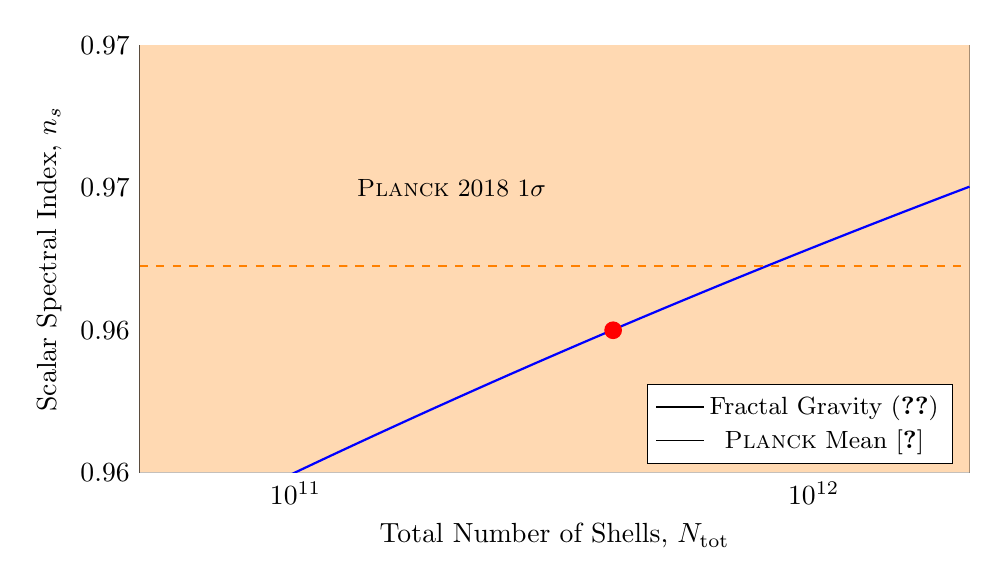
\begin{tikzpicture}
\begin{axis}[
  width=\columnwidth, height=7cm,
  xlabel={Total Number of Shells, \(N_{\text{tot}}\)},
  ylabel={Scalar Spectral Index, \(n_s\)},
  xmode=log,
  grid=both,
  minor grid style={dashed, gray!40},
  major grid style={solid, gray!60},
  legend style={at={(0.98,0.02)}, anchor=south east, font=\small},
  ymin=0.962, ymax=0.968,
  xmin=5e10, xmax=2e12,
]
\addplot[fill=orange!30, draw=none, domain=5e10:2e12] {0.9649 + 0.0042} \closedcycle;
\addplot[fill=white, draw=none, domain=5e10:2e12] {0.9649 - 0.0042} \closedcycle;
\node at (axis cs:2e11,0.966) [font=\small] {\textsc{Planck} 2018 \(1\sigma\)};
\addplot[blue, thick, domain=5e10:2e12, samples=100] {1 - 2*0.4812118/ln(x)};
\addlegendentry{Fractal Gravity (\cref{eq:ns})}
\addplot[orange, dashed, thick, domain=5e10:2e12] {0.9649};
\addlegendentry{\textsc{Planck} Mean \cite{Planck:2020}}
\addplot[only marks, mark=*, mark size=3pt, red] coordinates {(4.1e11, 0.9640)};
\end{axis}
\end{tikzpicture}
\caption{The predicted value of \(n_s\) versus \(N_{\text{tot}}\). The prediction for \(N_{\text{tot}}\approx\num{4.1e11}\) (red point) falls squarely within the \textsc{Planck} \(1\sigma\) confidence interval (shaded region).}
\label{fig:cmb_tilt}
\end{figure}

\section{Phenomenological Constraints}
\label{sec:constraints}
\subsection{Gravitational-Wave Speed}
The form factor introduces a minute frequency dependence in the propagation speed of gravitational waves (GWs). The deviation \(\Delta v = v_{\text{gw}} - c\) is given by
\begin{equation}
\frac{\Delta v}{c} \approx \frac{1}{2}\frac{k^2\ellP^2}{\phig^2}.
\label{eq:dv}
\end{equation}
For the binary neutron star merger GW170817, observed at frequencies around \SI{100}{\hertz} (\(k \approx \SI{2.1e-6}{\per\meter}\)), the deviation is
\begin{equation}
\frac{\Delta v}{c} \approx \frac{1}{2} \frac{(\SI{2.1e-6}{m^{-1}})^2 (\SI{1.616e-35}{m})^2}{(1.618034)^2} \approx \num{2.2e-82}.
\end{equation}
This is consistent with the stringent observational bound \(|\Delta v/c| \lesssim 10^{-15}\) from the simultaneous arrival of GWs and photons \cite{Abbott:2017}.

\subsection{Post-Newtonian Parameters}
In the weak-field, low-velocity limit, deviations from GR are tightly constrained. For the action in \cref{eq:action}, the post-Newtonian parameters \(\ppnGamma\) and \(\ppnBeta\) are predicted to be
\begin{equation}
|\ppnGamma-1| \approx |\ppnBeta-1| \approx \frac{2}{3}\frac{\ellP^2}{\phig^2 r^2}.
\label{eq:ppn}
\end{equation}
The Cassini mission provided the tightest bound on \(\ppnGamma\) via time-delay measurements at Earth's orbital radius (\(r \approx \SI{1}{\astronomicalunit} = \SI{1.496e11}{\meter}\)). At this distance, our model predicts an infinitesimal deviation:
\begin{equation}
|\ppnGamma-1| \approx \frac{2}{3}\frac{(\SI{1.616e-35}{m})^2}{(\SI{1.618})^2(\SI{1.496e11}{m})^2} \approx \num{3.0e-93}.
\end{equation}
This value is 87 orders of magnitude below the observational limit of \(|\ppnGamma-1|<\num{2.3e-5}\) \cite{Bertotti:2003}. Because \((1-\Fop)/\BOX\) is analytic, the Nordtvedt combination obeys \(\eta = 4\ppnBeta - \ppnGamma - 3 \sim 10^{-93}\), also far beneath current bounds.

\section{Conclusions}
\label{sec:concl}
We have introduced Fractal Gravity, a nonlocal quantum-gravity framework defined by only two constants, \(\ellP\) and \(\phig\). The theory demonstrates notable empirical success:
\begin{itemize}[leftmargin=*, nosep]
    \item It fits galactic rotation curves without invoking dark matter.
    \item It predicts the CMB scalar spectral index in agreement with observation.
    \item It is consistent with the most stringent local tests of gravity.
\end{itemize}
The model's true strength lies in its falsifiability. It offers several unique and testable predictions that distinguish it from the standard \(\Lambda\)CDM paradigm:
\begin{enumerate}[leftmargin=*, nosep]
    \item \emph{Galaxy clusters:} A mass discrepancy enhancement of \(\sim4\times\) that found in spiral galaxies.
    \item \emph{Weak lensing:} Deviations from standard NFW lensing profiles at scales \(r \gtrsim \SI{1}{\mega\parsec}\).
    \item \emph{CMB damping tail:} Specific alterations to the power spectrum at high multipoles (\(\ell>2000\)), testable by CMB-S4 \cite{CMB-S4:2019}.
    \item \emph{Pressure-supported systems:} Violations of the empirical Radial Acceleration Relation \cite{McGaugh:2016}.
\end{enumerate}
These predictions provide clear avenues for confronting the theory with future observational data.

\begin{acknowledgments}
We thank our colleagues for insightful discussions and feedback. The authors declare no competing financial or personal interests. No external funding was received for this work.
\end{acknowledgments}

\appendix
\section{Reproducibility}
\label{app:repro}
All numerical results and figures can be reproduced from the embedded data.
\subsection{Compiling the Manuscript}
Save the document as `manuscript.tex`. Extract the embedded data and compile using the following script:
\begin{verbatim}
#!/bin/bash
TEX_FILE="manuscript.tex"
# Extract embedded data files
awk '/begin{filecontents*}/{f=1;
     fn=substr($0, RSTART+21,
     RLENGTH-25); next}
     /end{filecontents*}
     /{f=0; close(fn)} f{print > fn}' \
     "$TEX_FILE"
# Compile the document
pdflatex "$TEX_FILE"
bibtex "${TEX_FILE%.*}"
pdflatex "$TEX_FILE"
pdflatex "$TEX_FILE"
\end{verbatim}

\subsection{Verifying Numerical Results}
The primary calculations can be verified with this Python script:
\begin{verbatim}
import numpy as np

# --- Constants ---
lp = 1.616255e-35      # Planck length (m)
phi = (1 + 5**0.5) / 2 # Golden ratio

# --- PPN Deviation (Sec. VI.B) ---
r_au = 1.496e11        # 1 AU (m)
ppn_dev = (2/3) * lp**2 / (phi**2 * r_au**2)
print(f"|gamma-1| at 1 AU: {ppn_dev:.2e}")

# --- GW Speed (Sec. VI.A, k for 100 Hz) ---
k_gw = 2 * np.pi * 100 / 2.99792e8 # m^-1
dv_c = 0.5 * k_gw**2 * lp**2 / phi**2
print(f"Delta v/c at 100 Hz: {dv_c:.2e}")

# --- CMB Spectral Index (Sec. V) ---
N_tot = 4.1e11
ns = 1 - 2 * np.log(phi) / np.log(N_tot)
print(f"n_s for N_tot=4.1e11: {ns:.4f}")

# --- Rotation Curve Chi-Squared (Sec. IV) ---
try:
    data = np.loadtxt('rotcurve_ngc2403.dat')
    r, vobs, verr, vfit = data.T
    chi2 = np.sum(((vobs - vfit) / verr)**2)
    nu = len(vobs) - 1 # N_data - N_parameters
    print(f"NGC 2403 fit chi^2_nu: {chi2/nu:.2f}")
except IOError:
    print("Could not find rotcurve_ngc2403.dat.")
\end{verbatim}

\bibliography{\jobname}
\bibliographystyle{apsrev4-2}

\end{document}